\documentclass[xcolor={usenames, svgnames}]{beamer}

\ifx\macrosHeader\undefined

%
% Styles
%
\newcommand{\subsubsubsection}[1]{{\bf #1} \vspace{0.5\baselineskip}}


%
% Copywriting
%
\newcommand{\bigO}[1]{\mathcal{O}{\left({ #1 }\right)}}

\newcommand{\hector}{HECToR}
\newcommand{\velocityverlet}{velocity Verlet}
\newcommand{\verletlist}{Verlet list}
\newcommand{\twobody}{two body}
\newcommand{\LennardJones}{Lennard-Jones}
\newcommand{\numa}{NUMA}

\newcommand{\openmp}{OpenMP}

\newcommand{\replicateddata}{replicated data}
\newcommand{\systolicloop}{systolic loop}
\newcommand{\sharedandreplicateddata}{shared and replicated data}
\newcommand{\replicatedsystolicloop}{replicated systolic loop}

\newcommand{\individualoperation}{
    \texttt{indi}\discretionary{-}{}{}\texttt{vidual\_}\discretionary{-}{}{}\texttt{operation}
}
\newcommand{\pairoperation}{
    \texttt{pair\_}\discretionary{-}{}{}\texttt{operation}
}

\newcommand{\EQN}[1]{Eqn.~(\ref{#1})}
\newcommand{\LST}[1]{Listing~\ref{#1}}
\newcommand{\FIG}[1]{Figure~\ref{#1}}
\newcommand{\SEC}[1]{Section~\ref{#1}}


\newcommand{\vZeroSpeedupCaption}[2]{
    {\bf Speedup vs. Cores} for the {\bf #1} implementation of the
    {\bf #2} method for systems of particles of size
    $N=512$ (red), $N=4096$ (green) and $N=32768$ (blue) and the
    function $f(x) = x$ (light red).
}

\newcommand{\vZeroSpeedupExplanation}[3]{
    #1 shows how the speedup of the #2 implementation of the
    #3 method scales with the number of cores available to the
    implementation.
    %
    This is presented for systems of particles of size
    $N=512$ shown in red, $N=4096$ shown in green
    and $N=32769$ shown in blue along with the function
    $f(x) = x$ shown in light red.
}

\newcommand{\vZeroTimeCaption}[3]{
    {\bf Time vs. Cores} for the {\bf #1} implementation of the
    {\bf #2} method for the total execution time (red),
    calculation execution time without MPI (green) and
    MPI execution time without calculations (blue)
    for an MD system of particles of size ${\bf N = {#3}}$.
}

\newcommand{\vOneSRTimeCaption}[3]{
    \vZeroTimeCaption{#1}{#2}{#3}
    %
    %The number cores presented is the number of MPI
    %processes used multiplied by the number of \openmp{} threads
    %available per MPI process.
}

\newcommand{\vZeroTimeExplanation}[5]{
    {#1}, {#2} and {#3}
    show how the execution time of the {#4} method
    for the {#5} scheme varies with
    the number of cores used for the simulation
    where $N$, the number of particles in the system, is
    512, 4096 and 32768 respectively.
    They present the cases where
    both MPI and calculations are performed (red)
        representing the total execution time;
    calculations are performed without MPI (green)
        representing the execution time of the simulation
        without communication effects; and
    MPI is performed without calculations (blue)
        representing the time taken up solely by the communications.
}

\newcommand{\vOneSRTimeExplanation}[5]{
    \vZeroTimeExplanation{#1}{#2}{#3}{#4}{#5}
    %
    In this graph, the cores listed represent the total possible cores
    $P = P_{MPI} \times{} P_{OMP}$ available to the implementation.
}


\def\macrosHeader{0}
\fi

\def\noepcc{1}
\def\noxcolor{1}
\ifx\packagesHeader\undefined

\usepackage{amsmath}

\usepackage{hyperref}

\usepackage{graphics}
\usepackage{graphicx}

\usepackage{epcc}

\usepackage[usenames, svgnames]{xcolor}
\usepackage{listings}

\usepackage{enumitem}

\usepackage{tikz}
\usepackage{tikz-uml}
\usetikzlibrary{shapes, arrows}


\def\packagesHeader{0}
\fi

\ifx\configurationHeader\undefined

%
% Set author, title and date
%
\author{\padraigoconbhui{}}
\title{\towardsexascalemd{}}
\date{\today}

\hypersetup{
    pdfauthor={\plainpadraigoconbhui{}},
    pdftitle={\towardsexascalemd{}}
}

%
% Set up hyperref package
%
\hypersetup{
    hidelinks
}



\lstset{frame=single, language=Fortran}
\lstset{
    commentstyle=\color{Blue},
    keywordstyle=\bf \color{Green},
    numbers=left,
    stepnumber=1
}
\lstset{morecomment=[s][\color{LimeGreen}]{PURE}{\ }}
\lstset{morecomment=[s][\color{LimeGreen}]{&}{\ }}


\usepackage{parskip}

\usepackage[font=footnotesize]{caption}



% Styles gratefully stolen from
% http://www.texample.net/tikz/examples/simple-flow-chart/
\tikzstyle{redcolor} = [red!80]
\tikzstyle{bluecolor} = [blue!20]
\tikzstyle{redfill} = [fill=red!80]
\tikzstyle{bluefill} = [fill=blue!20]
\tikzstyle{decision} = [diamond, draw, bluefill, 
    text width=4.5em, text badly centered, node distance=3cm, inner sep=0pt]
\tikzstyle{block} = [rectangle, draw, bluefill, 
    text width=5em, text centered, rounded corners, minimum height=4em]
\tikzstyle{line} = [draw, -latex', rounded corners, thick]


\def\configurationHeader{0}
\fi


\title[Exascale MD]{Towards Exascale Molecular Dynamics}
\author[P. O Conbhui]{P\'{a}draig \'{O} Conbhu\'{\i}}
\date[August 2013]{August 27, 2013}

\begin{document}

\begin{frame}[plain]
    \titlepage
\end{frame}

% Introduction to MD
% Introduction to Truncation, Chaos
% Introduction to parallel schemes
% % RD
% % SL
% % SRD
% % RSL

\section{Introduction to MD}

\begin{frame}{The Hamiltonian}
    Hamiltonian for twobody potential:
    \begin{equation}
        H = \sum_{i=1}^N \frac{\vec{p}_i^{,2}}{2 m}
            + \sum_{i=1}^N \sum_{j<i}^N V(\vec{x}_i, \vec{x}_j)
    \end{equation}
    
    Equations of Motion:
    \begin{equation}
        m_i \vec{a}_i = -\sum_{\substack{j=1\\j\ne{}i}}^N
                        \vec{\nabla}_i V(\vec{x}_i, \vec{x}_j)
    \end{equation}
\end{frame}


\begin{frame}{The Velocity Verlet Algorithm}
    Discretisation using the \velocityverlet{} scheme:
    \begin{subequations}
    \label{eqn:velocity_verlet_scheme}
    \begin{align}
        \vec{v}_i(t + \tfrac{1}{2} h) &=
            \vec{v}_i(t) + \tfrac{1}{2}\vec{a}_i h
        \label{eqn:velocity_verlet_v1_update}
        \\
        \vec{x}_i(t + h) &=
            \vec{x}_i(t) + \vec{v}_i(t + \tfrac{1}{2} h) h
        \label{eqn:velocity_verlet_position_update}
        \\
        m_i \vec{a}_i(t + h) &=
            - \sum_{\substack{j=1\\j\ne{}i}}^N
                \vec{\nabla}_i V(\vec{x}_i(t+h), \vec{x}_j(t+h))
        \label{eqn:velocity_verlet_force_eval}
        \\
        \vec{v}_i(t+h) &=
            \vec{v}_i(t + \tfrac{1}{2} h) + \tfrac{1}{2} \vec{a}_i(t + h) h
        \label{eqn:velocity_verlet_v2_update}
    \end{align}
    \end{subequations}

    Force evaluation $\rightarrow{}$ $\bigO{N^2}$ per time step.
\end{frame}


\begin{frame}{Tackling Force Evaluation}
    Some approximations:
    \begin{itemize}
        \item Truncation
        \item Fast Multipole
        \item P${}^3$M
    \end{itemize}

    Some parallel schemes:
    \begin{itemize}
        \item Domain Distribution
        \item Replicated Data
        \item Systolic Loop
    \end{itemize}

    How well can force evaluations be parallelised without
    any approximations?
\end{frame}


\section{Parallel Schemes}

\begin{frame}{Schemes Of Interest}
    Two main schemes studied:
    \begin{itemize}
        \item Replicated Data
        \item Systolic Loop
    \end{itemize}

    Two improved schemes studied
    \begin{itemize}
        \item Shared And Replicated Data
        \item Replicated Systolic Loop
    \end{itemize}
\end{frame}


\newcommand{\rdpic}{
    \begin{center}
        \scalebox{0.75}{
            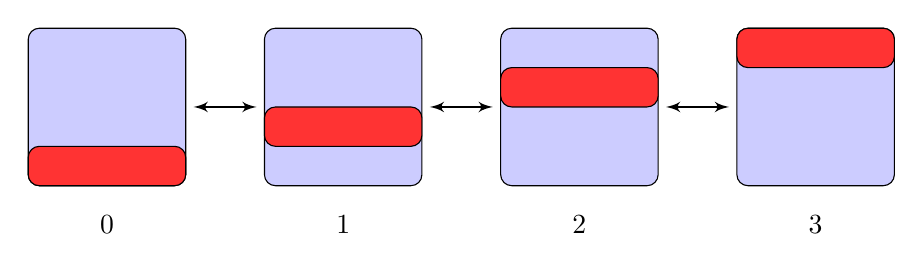
\begin{tikzpicture}[scale=.5]
                % Draw replicated blocks and force areas
                \foreach \n in {0,...,3} {
                    \draw [block] (6*\n,0) rectangle (6*\n+4,4);
                    \draw [block, redfill] (6*\n,\n) rectangle (6*\n+4,\n+1);
                }
                %
                % Draw arrows
                \foreach \n in {0,...,2} {
                    \draw [latex'-latex', thick] (6*\n+4.2,2) -- (6*\n+5.8,2);
                }
                %
                % Draw text
                \foreach \n in {0,...,3} {
                    \node at (2 + 6*\n, -1) {\n};
                }
            \end{tikzpicture}
        }
    \end{center}
}

\begin{frame}{Replicated Data}
    \rdpic{}

    \begin{itemize}
        \item Full system replicated on each process
        \item Each process updates $N/P$ particles
        \item Processes share results to synchronise lists
        \item Calculation: $N^2/P$
        \item Communications: $N\log{P}$
    \end{itemize}
\end{frame}


\begin{frame}{Shared And Replicated Data}
    \rdpic{}

    \begin{itemize}
        \item Full system replicated on each {\bf MPI} process
        \item Each {\bf MPI} process updates $N/P_{MPI}$ particles
        \item Each {\bf MPI} processes spawns $P_{OMP}$ {\bf \openmp} threads
        \item Each {\bf \openmp{}} thread updates
            $N/(P_{MPI}\times{}P_{OMP})$ particles.
        \item {\bf MPI} processes share results to synchronise lists.
        \item Calculation: $N^2/(P_{MPI}\times{}P_{OMP})$
        \item Communications: $N\log{P_{MPI}}$
    \end{itemize}
\end{frame}


\newcommand{\slpic}{
    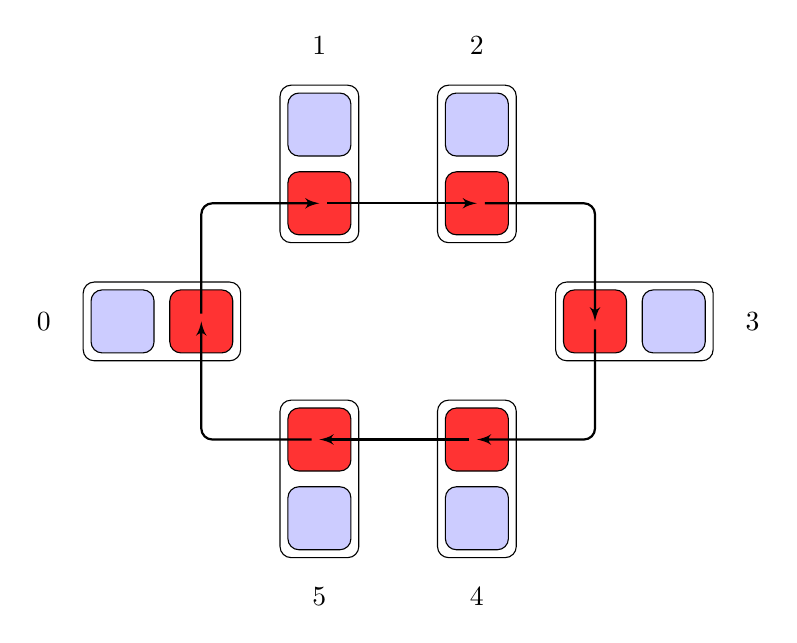
\begin{tikzpicture}
        %
        % Draw bounding boxes
        \draw [draw, rounded corners] (-0.5,0) rectangle +(2, 1);
        %
        \draw [draw, rounded corners] (2,1.5) rectangle +(1, 2);
        \draw [draw, rounded corners] (4,1.5) rectangle +(1, 2);
        %
        \draw [draw, rounded corners] (5.5,0) rectangle +(2, 1);
        %
        \draw [draw, rounded corners] (4,-0.5) rectangle +(1, -2);
        \draw [draw, rounded corners] (2,-0.5) rectangle +(1, -2);
        %
        % Draw outer ring
        \foreach \xy in {
            {(-0.5,0)},
            {(2,2.5)}, {(4,2.5)},
            {(6.5,0)},
            {(4,-2.5)}, {(2,-2.5)}
        } {
            \draw [block, bluefill]
                {\xy+(0.1,0.1)} rectangle +(0.9, 0.9);
        }
        %
        % Draw inner ring
        \foreach \xy in {
            {(0.5,0)},
            {(2,1.5)}, {(4,1.5)},
            {(5.5,0)},
            {(4,-1.5)}, {(2,-1.5)}
        } {
            \draw [block, redfill]
                {\xy+(0.1,0.1)} rectangle +(0.9, 0.9);
        }
        %
        % Draw circle
        \newcommand{\off}{0.1}
        \path [line] (1, 0.5+\off) |- +(1.5, 1.5-\off);
        %
        \path [line] (2.5+\off, 2) -- +(2-\off, 0);
        \path [line] (4.5+\off, 2) -| +(1.5-\off, -1.5);
        %
        \path [line] (6, 0.5-\off) |- +(-1.5, -1.5+\off);
        %
        \path [line] (4.5-\off, -1) -- +(-2+\off, 0);
        \path [line] (2.5-\off, -1) -| +(-1.5+\off, +1.5);
        %
        % Draw labels
        \foreach \xy/\n in {
            {(-1,0.5)}/0,
            {(2.5,4)}/1, {(4.5,4)}/2,
            {(8,0.5)}/3,
            {(4.5,-3)}/4, {(2.5,-3)}/5
        } {
            \node at \xy {\n};
        }
    \end{tikzpicture}
}


\begin{frame}{Systolic Loop}
    \begin{center}
        \resizebox{0.5\textwidth}{!}{
            \slpic{}
        }
    \end{center}

    \begin{itemize}
        \item Distribute system across $P$ processes
        \item Pass packets of $N/P$ particles around the ring
        \item Perform $P$ list comparisons of $N/P$ particles
        \item Calculation: $\bigO{P(N/P)^2} = \bigO{N^2/P}$
        \item Communications: $\bigO{N + P}$.
    \end{itemize}
\end{frame}

\begin{frame}{Replicated Systolic Loop}
    \begin{center}
        \begin{minipage}{0.3\textwidth}
                \resizebox{\textwidth}{!}{
                    \slpic{}
                }
        \end{minipage}%
        \begin{minipage}{0.3\textwidth}
                \resizebox{\textwidth}{!}{
                    \slpic{}
                }
        \end{minipage}%
        \begin{minipage}{0.3\textwidth}
                \resizebox{\textwidth}{!}{
                    \slpic{}
                }
        \end{minipage}
    \end{center}

    \begin{itemize}
        \item Decompose $P$ processes into 2d $S\times{}R$ topology
        \item Distribute system across systolic loop of size $S$
        \item Copy across $R$ replica rings
        \item Each replica performs $S/R$ of the systolic pulses
        \item Perform $S/R$ list comparisons of $N/S$ particles
        \item Reduce results over $R$ replicas
        \item Calculation:
            $\bigO{(S/R)(N/S)^2} = \bigO{N^2/(SR)} = \bigO{N^2/P}$
        \item Communications: $\bigO{N/R + S/R + (N/S)\log{R} + \log{R}}$
    \end{itemize}
\end{frame}

\end{document}
